\todo[inline,color=yellow]{Listar equipamentos (modelo e número de identificação quando possível) e componentes (valores nominais) utilizados.}

\begin{figure}
	\centering
	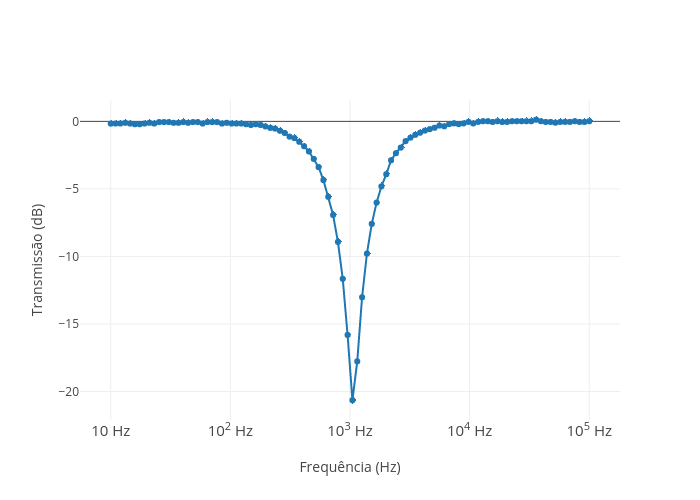
\includegraphics[width=0.9\textwidth]{figuras/diagrama-bode.png}
	\caption{
    	Diagrama de Bode
	}
    \label{fig:frog}
\end{figure}

\begin{center}
	\begin{tabular}{l|c}
    	\bfseries Frequência (Hz) & \bfseries Transmitância (dB)
     	\csvreader[head to column names]{dados/parte2.csv}{}
      	{\\\hline \freq & \TdB}
	\end{tabular}
\end{center}